\documentclass[11pt, oneside]{report}   	% use "amsart" instead of "article" for AMSLaTeX format
\usepackage[latin1]{inputenc} 
\usepackage[T1]{fontenc}
\usepackage{geometry}                		% See geometry.pdf to learn the layout options. There are lots.
\geometry{letterpaper}                   		% ... or a4paper or a5paper or ... 
%\geometry{landscape}                		% Activate for rotated page geometry
%\usepackage[parfill]{parskip}    		% Activate to begin paragraphs with an empty line rather than an indent
\usepackage{graphicx}				% Use pdf, png, jpg, or eps§ with pdflatex; use eps in DVI mode
								% TeX will automatically convert eps --> pdf in pdflatex		

\usepackage{xcolor}
\usepackage{amssymb}
\usepackage{listings}
\usepackage{caption}
\usepackage{hyperref}
\usepackage[scaled=0.85]{beramono}
\usepackage[scaled]{beraserif}
\usepackage[scaled]{berasans}

\renewcommand*\familydefault{\rmdefault} 
 
\lstset{
	numbers=left,
	basicstyle=\ttfamily\scriptsize,
	breakatwhitespace=false,
	frame=single,
  	breaklines=true, 
  	captionpos=t, 
	numbersep=10pt,
	numberstyle=\tiny,
	showspaces=false,
	tabsize=2,	
	language=C,
	label=DescriptiveLabel,
 	commentstyle=\color{gray},
 	keywordstyle=\color{blue}
}


\usepackage{titling}
\newcommand{\subtitle}[1]{
  \posttitle{
    \par\end{center}
    \begin{center}\large#1\end{center}
    \vskip0.5em}
}
\DeclareCaptionFormat{listing}{\rule{\dimexpr\textwidth+17pt\relax}{0.4pt}\vskip1pt#1#2#3}

\title{Matrix Multiplication with POP}
\subtitle{Performance analysis of a distributed matrix multiplication program}
\author{Alshweiki Mhd Ali \thanks{\ mhdali.alshweiki@master.hes-so.ch}\\ 
Gugger Jo�l \thanks{\ joel.gugger@master.hes-so.ch}\\ 
Marguet Steve-David \thanks{\ stevedavid.marguet@master.hes-so.ch} \\ \\ user: ggroup20@grid11}
\date{\today}

\begin{document}
\maketitle


\pagenumbering{gobble}



\begin{abstract}

The objective of this lab is to execute and to analyse the performances of a parallel square matrices multiplication program written in POP-C++ and in POP-Java. As for the MPI/OpenMP lab, these programs compute square matrices multiplication, i.e. the product $A \times B = R$ where $A$, $B$ and $R$ are $N \times N$ matrices (square matrix).

The program uses a � Master/Worker � approach. The master prepares the matrices, creates the workers (POP-C++ or POP-Java parallel objects), sends the work to do to each workers, waits for the partial result of each worker and finally reconstructs the $R$ matrix.

The algorithm behaves similarly to the one of the MPI/OpenMP lab by dividing the matrix $A$ in several blocks of lines and the matrix $B$ in several blocks of columns.

\end{abstract}


\pagenumbering{arabic}

\chapter{Computation of "sequential" references times}
The so-called sequential reference time is the time we used to do the computation of the whole matrices, using only one worker and four cores.

\lstinputlisting[language=bash,numbers=none,caption={Sequential results},basicstyle=\ttfamily\tiny,]{./files/sequential_time.sh}

\newpage

\begin{figure}
    \begin{center}
        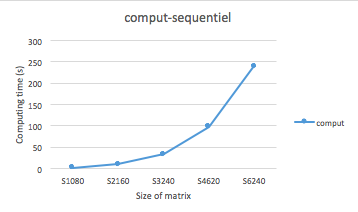
\includegraphics[width=300pt]{Plots/Comput-seq.png}
        \caption{Sequential computing time}
        \label{fig:Sequential computing time}
    \end{center}
\end{figure}

\begin{figure}
    \begin{center}
        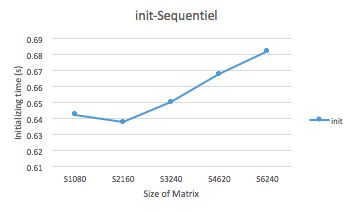
\includegraphics[width=300pt]{Plots/Init-seq.png}
        \caption{Sequential computing - Initialization time}
        \label{fig:Sequential computing - Initialization time}
    \end{center}
\end{figure}

\begin{figure}
    \begin{center}
        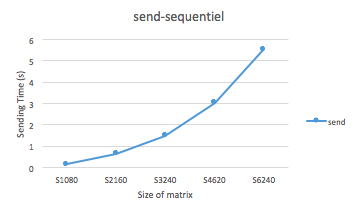
\includegraphics[width=300pt]{Plots/Send-seq.png}
        \caption{Sequential computing - Sending time}
        \label{fig:Sequential computing - Sending time}
    \end{center}
\end{figure}

\begin{figure}
    \begin{center}
        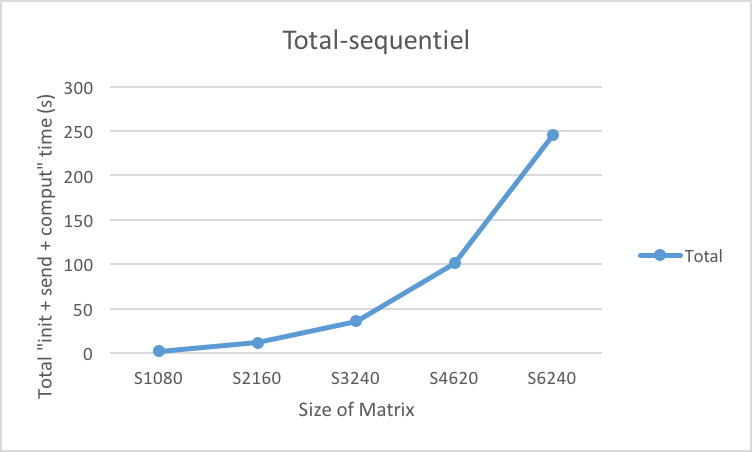
\includegraphics[width=300pt]{Plots/Total-seq.png}
        \caption{Sequential computing - Total time}
        \label{fig:Sequential computing - Total time}
    \end{center}
\end{figure}

\chapter{Computation of parallel times}
Each group will have to compute for five different sizes of matrices ($N$), the time for five different numbers of workers ($W$). Our group will make computations for this sizes:

\vspace{1cm}
\[
\begin{tabular}{|r|}
\hline
Matrix sizes ($N$) \\
\hline
1080	\\
2160	\\
3240	\\
4620	\\
6240	\\
\hline
\end{tabular}
\]

\vspace{1cm}
\[
\begin{tabular}{|c|r|}
\hline
Workers ($W$) & $= LxC$ \\
\hline
2	& $=1x2$\\
4	& $=2x2$ \\
6	& $=2x3$ \\
9	& $=3x3$ \\
10	& $=5x2$ \\
\hline
\end{tabular}
\]

\newpage

We had some difficulties to execute our script correctly. The first time, the script haven't be executed because relative path. The second time, the script ran but we compute only 25 calculs. We have made only one size by worker size. 


\lstinputlisting[language=bash,caption={Cron job}]{./files/crontab.sh}

\newpage

This version is the third version that execute the 100 calculation we missed. This why in each size we have a commented line.


\lstinputlisting[language=bash,caption={Final bash script}]{./files/runme.sh}

\begin{figure}
    \begin{center}
        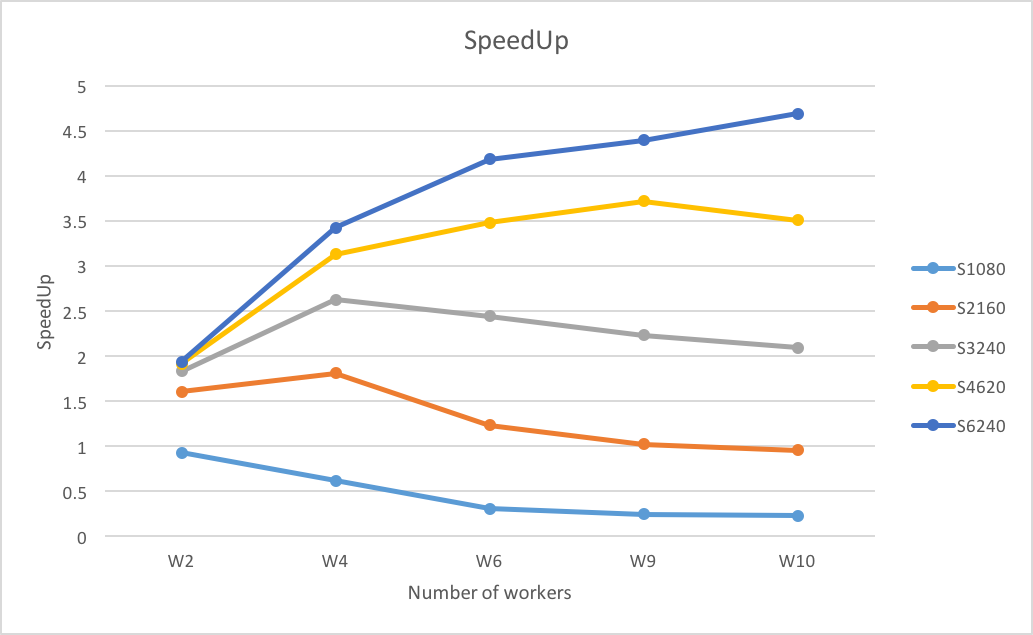
\includegraphics[width=300pt]{Plots/SpeedUp.png}
        \caption{SpeedUp}
        \label{fig:SpeedUp}
    \end{center}
\end{figure}

\begin{figure}
    \begin{center}
        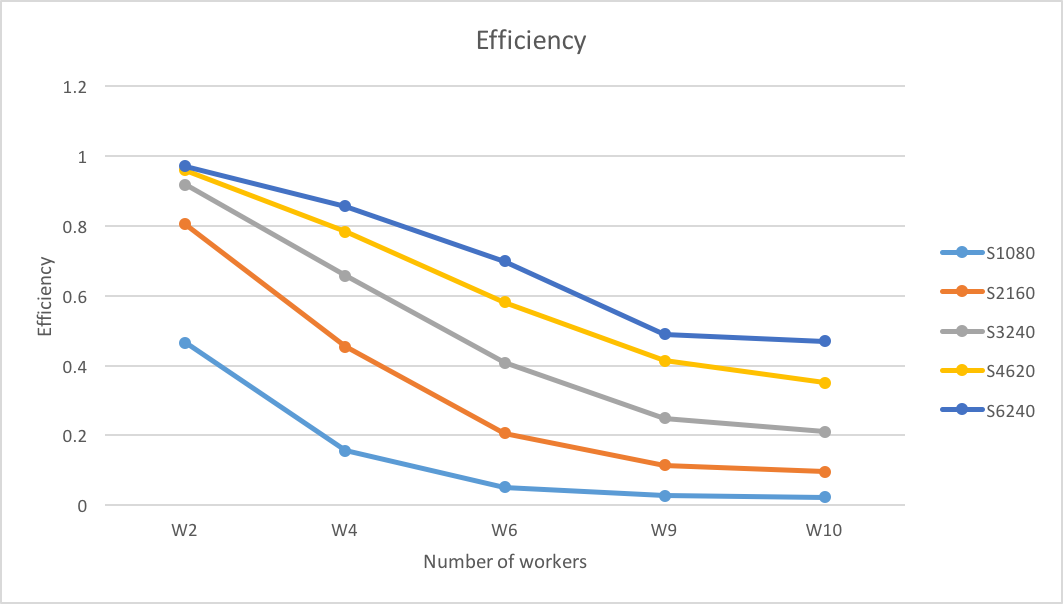
\includegraphics[width=300pt]{Plots/Efficiency.png}
        \caption{Efficiency}
        \label{fig:Efficiency}
    \end{center}
\end{figure}

\newpage

\begin{abstract}
\begin{center}
The sources of the project are available on GitHub at the following address: \\
\href{https://github.com/Alshweiki/ProgAlg-Lab2}{https://github.com/Alshweiki/ProgAlg-Lab2}
\end{center}
\end{abstract}


\end{document}  











